% AML-RL Framework Architecture Blueprint
% Compile with pdflatex or XeLaTeX

\documentclass[11pt,a4paper]{article}

% Packages
\usepackage[utf8]{inputenc}
\usepackage[T1]{fontenc}
\usepackage{geometry}
\usepackage{amsmath,amssymb}
\usepackage{algorithm}
\usepackage{algorithmic}
\usepackage{graphicx}
\usepackage{booktabs}
\usepackage{multirow}
\usepackage{xcolor}
\usepackage{hyperref}
\usepackage{tikz}
\usepackage{listings}
\usepackage{subcaption}

\geometry{margin=1in}

% Colors
\definecolor{codegreen}{rgb}{0,0.6,0}
\definecolor{codegray}{rgb}{0.5,0.5,0.5}
\definecolor{codepurple}{rgb}{0.58,0,0.82}
\definecolor{backcolour}{rgb}{0.95,0.95,0.92}

% Code listing style
\lstdefinestyle{pythonstyle}{
    backgroundcolor=\color{backcolour},
    commentstyle=\color{codegreen},
    keywordstyle=\color{magenta},
    numberstyle=\tiny\color{codegray},
    stringstyle=\color{codepurple},
    basicstyle=\ttfamily\footnotesize,
    breakatwhitespace=false,
    breaklines=true,
    captionpos=b,
    keepspaces=true,
    numbers=left,
    numbersep=5pt,
    showspaces=false,
    showstringspaces=false,
    showtabs=false,
    tabsize=2
}
\lstset{style=pythonstyle}

\title{\textbf{AML-RL: A Modular Framework for\\Graph-Based Anti-Money Laundering Detection}}
\author{Framework Architecture Blueprint v1.0}
\date{\today}

\begin{document}

\maketitle

\begin{abstract}
We present \textbf{AML-RL}, the reference architecture we built to instantiate \textbf{RL-Guard}---our production gateway for safe reinforcement learning---inside a graph-based anti-money laundering (AML) environment. The framework combines three ingredients: (i) a declarative \emph{pipeline factory} that assembles datasets, feature engineering, encoders, agents, and trainers from a single configuration; (ii) a plug-and-play catalog of graph neural encoders (GraphSAGE, GAT, RMGANets) and DQN/QR-DQN agents that share a uniform audit surface; and (iii) the RL-Guard safety, audit, and deployment modules that sit between any trained policy and downstream banking systems. Rather than advertising a specific F1 score, this document details how modularity, configuration immutability, and guardrails let us iterate on encoders, agents, and datasets (including differing class priors such as Elliptic's ``include-unlabeled'' toggle) without rewriting infrastructure. The blueprint is meant for researchers and engineers who need to plug new components into the framework while keeping RL-Guard's compliance guarantees intact.
\end{abstract}

\section{Introduction}

Traditional AML systems rely on static rule-based detection or supervised machine learning, limiting adaptability to evolving fraud patterns. \textbf{AML-RL} addresses these limitations through:

\begin{itemize}
    \item \textbf{Graph-based representation}: Transaction networks as directed graphs
    \item \textbf{Deep reinforcement learning}: Adaptive pattern detection through experience
    \item \textbf{Modular architecture}: Plug-and-play components for rapid experimentation
    \item \textbf{Production readiness}: GPU acceleration, distributed training, API serving
\end{itemize}

\subsection{Key Contributions}

\begin{enumerate}
    \item \textbf{Gateway alignment}: Formal interface between RL-Guard (safety engine, audit stream, safe deployment) and any AML policy built by the factory. Every encoder/agent combination emits the same artefacts (state embeddings, auxiliary logits, Q-value envelopes) so RL-Guard can enforce business directives without bespoke code.
    \item \textbf{Pipeline factory}: Declarative configs drive data sampling, feature engineering, encoder selection, agent wiring, and trainer settings. A single JSON/CLI contract can switch from AMLNet$\rightarrow$Elliptic, GraphSAGE$\rightarrow$RMGANets, or DQN$\rightarrow$QR-DQN.
    \item \textbf{Pluggable components}: Graph encoders (SAGE, GAT, RMGANets~\cite{rmganets2024}), reinforcement-learning heads (dueling DQN, QR-DQN with CVaR policies~\cite{dabney2018distributional}), and loss modules (simplified vs.\ improved multi-branch) are imported via factories with shared type hints and tests.
    \item \textbf{Dataset controls}: Built-in toggles (e.g., \texttt{--include-unlabeled} for Elliptic/Elliptic2) manage class priors and sampling without code edits, ensuring experiments reflect production priors before policies reach RL-Guard.
    \item \textbf{Documentation + automation}: The framework ships with extensibility notes, config validators, smoke tests, and CLI tooling so contributors can add new datasets/encoders while keeping RL-Guard's interface contract intact.
\end{enumerate}

\section{Framework Architecture}

\subsection{System Overview}

The AML-RL framework consists of six modular layers (Figure~\ref{fig:architecture}) that ultimately feed RL-Guard's gateway API:

\begin{enumerate}
    \item \textbf{Data Layer}: Dataset loaders and graph construction
    \item \textbf{Feature Extraction Layer}: 20-dimensional feature engineering
    \item \textbf{Graph Encoding Layer}: GNN-based state representation
    \item \textbf{RL Layer}: Environment and agent interactions
    \item \textbf{Training Layer}: Loss functions and optimization
    \item \textbf{Evaluation Layer}: Metrics and baselines, plus the REST/audit contract consumed by RL-Guard
\end{enumerate}

\begin{figure}[htbp]
\centering
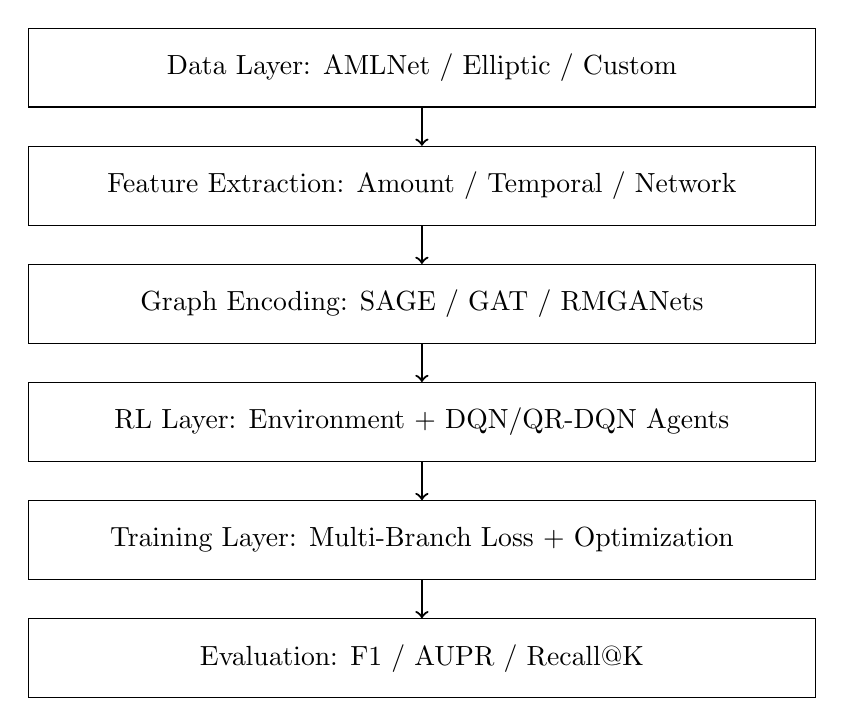
\begin{tikzpicture}[
    node distance=1.5cm,
    layer/.style={rectangle, draw, minimum width=10cm, minimum height=1cm, align=center},
    arrow/.style={->, thick}
]
    \node[layer] (data) {Data Layer: AMLNet / Elliptic / Custom};
    \node[layer, below of=data] (features) {Feature Extraction: Amount / Temporal / Network};
    \node[layer, below of=features] (gnn) {Graph Encoding: SAGE / GAT / RMGANets};
    \node[layer, below of=gnn] (rl) {RL Layer: Environment + DQN/QR-DQN Agents};
    \node[layer, below of=rl] (train) {Training Layer: Multi-Branch Loss + Optimization};
    \node[layer, below of=train] (eval) {Evaluation: F1 / AUPR / Recall@K};

    \draw[arrow] (data) -- (features);
    \draw[arrow] (features) -- (gnn);
    \draw[arrow] (gnn) -- (rl);
    \draw[arrow] (rl) -- (train);
    \draw[arrow] (train) -- (eval);
\end{tikzpicture}
\caption{AML-RL Framework Architecture}
\label{fig:architecture}
\end{figure}

\subsection{Factory Pattern Design}

All major components use the factory pattern for modularity:

\begin{lstlisting}[language=Python, caption=Factory Pattern Example]
# Plug-and-play GNN encoders
encoder = GNNEncoderFactory.create(
    type="rmganets",  # or "sage", "gat", custom
    node_feature_dim=12,
    embedding_dim=64
)

# Plug-and-play RL agents
agent = RLAgentFactory.create(
    type="qrdqn",  # or "dqn", "ddqn", custom
    state_dim=80,
    action_dim=6
)

# Plug-and-play loss functions
loss = LossFactory.create(
    type="multibranch",  # or "simple", custom
    lambda_branch=0.25,
    epsilon_dqn=0.4
)
\end{lstlisting}

\subsection{Relation to Existing RL Frameworks}

Libraries such as RLlib, Stable-Baselines3, or CleanRL offer excellent algorithmic implementations but stop at the training loop.\cite{ray2025rllib} AML-RL sits \emph{above} those libraries: we still rely on PyTorch+Gymnasium primitives, yet we add
\begin{itemize}
    \item \textbf{Gateway awareness}: every component emits the metadata RL-Guard needs for safety/audit enforcement. RLlib policies do not expose fraud-specific payloads or per-branch logits out of the box.
    \item \textbf{Domain-specific data factory}: AML datasets require entity-disjoint splits, fraud-aware sampling, and toggles such as \texttt{--include-unlabeled}. RLlib expects generic vectorized observations and leaves data governance to the user.
    \item \textbf{Immutable configuration + automation}: configs double as deployment manifests; RL-Guard refuses checkpoints that do not match the stored config hash. Commodity libraries do not couple policies with compliance proofs.
\end{itemize}
Thus AML-RL complements, rather than replaces, algorithm libraries: it wraps whichever encoder/agent we pick in a standards-compliant harness so RL-Guard can safely mediate production traffic.
\subsection{RL-Guard Integration Contract}

Every artefact produced by the factory must satisfy RL-Guard's gateway contract:
\begin{itemize}
    \item \textbf{Action API}: Policies expose \texttt{/v1/propose\_action} with inputs \{state embedding, auxiliary logits, timestamp\} and outputs \{action, confidence, fraud explanation\}. RL-Guard injects business directives (e.g., ``block $>$30\% flags'') before the action reaches downstream systems.
    \item \textbf{Safety Hooks}: Feature extractors and encoders must emit fraud labels, branch logits, and Q-distributions so the Safety Engine can run predicate checks (rate limits, monotonicity, regulatory rules).
    \item \textbf{Audit Payloads}: Trainers log deterministic metadata (config hash, dataset snapshot, seed) that RL-Guard stores alongside each decision, enabling immutable replay.
    \item \textbf{Deployment Artefacts}: Checkpoints follow a naming convention (\texttt{outputs/<run>/checkpoints/checkpoint\_epXXXX.pt}) with embedded config JSON so the safe-deployment module can compare candidate vs.\ golden runs before promotion.
\end{itemize}

Because these hooks are enforced at the type level, RL-Guard does not need to know which encoder/agent produced the policy---any compliant component can be swapped without adjusting safety code.
\section{Module Reference}

\subsection{Data Layer}

\begin{table}[htbp]
\centering
\caption{Dataset Loaders}
\label{tab:datasets}
\begin{tabular}{@{}llll@{}}
\toprule
\textbf{Dataset} & \textbf{File} & \textbf{Paper Ref} & \textbf{Status} \\
\midrule
AMLNet~\cite{amlnet2024} & \texttt{datasets/amlnet.py} & AMLNet §3.1 & ✓ \\
Elliptic~\cite{elliptic2019} & \texttt{datasets/elliptic.py} & Elliptic §2 & ✓ \\
Synthetic & \texttt{datasets/synthetic.py} & Custom & ✓ \\
\bottomrule
\end{tabular}
\end{table}

\textbf{Graph Construction}: NetworkX directed graph with:
\begin{itemize}
    \item \textbf{Nodes}: Accounts with 20-dimensional features
    \item \textbf{Edges}: Transactions with timestamps $t_i$
    \item \textbf{Temporal constraint}: $t_{next} \geq t_{current}$ (no time travel)
\end{itemize}

\textbf{Class-Prior Toggle (Elliptic/Elliptic2)}: The dataset loader exposes an \texttt{include\_unlabeled} flag (also reachable via \texttt{--include-unlabeled} on the CLI). When enabled, the loader retains ``unknown'' clusters so the fraud prior reflects the original $\approx$2\% reported in the Elliptic release~\cite{elliptic2019}. RL-Guard enforces that this flag is ignored for AMLNet/Synthetic datasets to prevent misconfiguration. For context, recent graph-AML systems such as LaundroGraph and DELATOR~\cite{cardoso2022laundrograph,assumpcao2022delator} also operate on these datasets but lack a gateway-aware mechanism for managing class priors.

\subsection{Feature Extraction Layer}

\textbf{20-dimensional Feature Vector} (enhanced from AMLNet's 12-dim):

\begin{equation}
\mathbf{x}_i = [\mathbf{x}^{amt}_i, \mathbf{x}^{temp}_i, \mathbf{x}^{net}_i] \in \mathbb{R}^{20}
\end{equation}

Where:
\begin{itemize}
    \item $\mathbf{x}^{amt}_i \in \mathbb{R}^3$: Amount features (log(sent), log(received), balance)
    \item $\mathbf{x}^{temp}_i \in \mathbb{R}^{10}$: Temporal features (velocity, business hours, periodicity)
    \item $\mathbf{x}^{net}_i \in \mathbb{R}^7$: Network features (degree, clustering, centrality)
\end{itemize}

\subsubsection{Temporal Features (AMLNet Algorithm 2)}

Following AMLNet's Algorithm 2 \cite{amlnet2024}:

\begin{algorithm}[H]
\caption{Temporal Feature Extraction}
\begin{algorithmic}[1]
\REQUIRE Transaction history $T_i$ for account $i$, time window $\Delta t$
\STATE $V_i \gets$ transactions in window $[t - \Delta t, t]$
\STATE $velocity \gets |V_i| / \Delta t$ \COMMENT{Line 3-4}
\STATE $business\_hours \gets \mathbb{1}_{9 \leq hour(t) \leq 17}$ \COMMENT{Line 5}
\STATE $periodicity \gets FFT(timestamps)$ \COMMENT{Line 6-7}
\RETURN $\mathbf{x}^{temp}_i$
\end{algorithmic}
\end{algorithm}

\subsubsection{Network Features (PyG-Accelerated)}

\textbf{Improvement over AMLNet}: PyG GPU acceleration

\begin{table}[htbp]
\centering
\caption{Network Feature Complexity}
\begin{tabular}{@{}lcc@{}}
\toprule
\textbf{Feature} & \textbf{NetworkX} & \textbf{PyG (Ours)} \\
\midrule
Degree & $O(n^2)$ & $O(m)$ \\
Centrality & $O(n^3)$ & $O(m)$ \\
Clustering & $O(n^3)$ & $O(n^3)$ (fallback) \\
\bottomrule
\end{tabular}
\end{table}

\subsection{Graph Encoding Layer}

\subsubsection{RMGANets Architecture}

Our complete implementation of RMGANets \cite{rmganets2024} with all four modules:

\begin{table}[htbp]
\centering
\caption{RMGANets Module Implementation}
\label{tab:rmganets_modules}
\begin{tabular}{@{}llccc@{}}
\toprule
\textbf{Module} & \textbf{File} & \textbf{LOC} & \textbf{Equations} & \textbf{Status} \\
\midrule
Att-GCM & \texttt{att\_gcm.py} & 169 & 1-7 & ✓ \\
To-GCM & \texttt{to\_gcm.py} & 135 & 8-9 & ✓ \\
HyGCM & \texttt{hy\_gcm.py} & 150 & 10-11 & ✓ \\
Fusion & \texttt{fusion.py} & 88 & 12 & ✓ \\
Multi-Branch & \texttt{multi\_branch\_loss.py} & 400 & 14 & ✓ \\
\bottomrule
\end{tabular}
\end{table}

\paragraph{Att-GCM (Attention-Relation Graph Convolution)}

Equations from RMGANets §3.2.1:

\begin{align}
\mathbf{x}_{norm} &= \text{BatchNorm}(\mathbf{x}) \tag{Eq 1} \\
\mathbf{H}^{(1)} &= \sigma(\tilde{\mathbf{A}} \cdot \Phi(\mathbf{x}) \cdot \mathbf{W}) \tag{Eq 2} \\
A_{ij} &= \|\delta(\mathbf{x}_i) - \delta(\mathbf{x}_j)\|_2 \tag{Eq 5-6}
\end{align}

Where $\delta(\cdot)$ is 8-head multi-head attention output.

\textbf{Subgraph Splitting} (Eq 7):

\begin{align}
\mathcal{E}^{\nabla h} &= \{(i,j) : A_{ij} \geq T_1\} \quad \text{(high similarity, $T_1=0.7$)} \\
\mathcal{E}^{\nabla m} &= \{(i,j) : T_2 \leq A_{ij} < T_1\} \quad \text{(medium)} \\
\mathcal{E}^{\nabla l} &= \{(i,j) : A_{ij} < T_2\} \quad \text{(low similarity, $T_2=0.3$)}
\end{align}

\paragraph{To-GCM (Adaptive Topology Graph Convolution)}

Equations from RMGANets §3.2.2:

\begin{multline}
\mathbf{H}_1 = \sigma(\mathbf{A}^{\nabla hm} \odot \mathbf{H} \odot \mathbf{W}_1) \otimes \\
\left[\sigma(\mathbf{A}^{\nabla h} \odot \mathbf{H} \odot \mathbf{W}_2) \oplus \sigma(\mathbf{A}^{\nabla m} \odot \mathbf{H} \odot \mathbf{W}_3)\right] \tag{Eq 8}
\end{multline}

With shared node weighting (Eq 9):
\begin{equation}
w_{ij} = \begin{cases}
2.0 & \text{if } (i,j) \in \mathcal{E}^{\nabla h} \cap \mathcal{E}^{\nabla m} \\
1.0 & \text{otherwise}
\end{cases}
\end{equation}

\paragraph{HyGCM (Hybrid Enhanced Graph Convolution)}

Equations from RMGANets §3.2.3:

\begin{align}
\mathbf{H}_2 &= \sigma(\mathbf{A}^{\nabla hl} \odot \mathbf{H} \odot \mathbf{W}_4) + \text{LAM}(\cdot) \tag{Eq 10} \\
\text{LAM} &= \mathbf{h}_{low} + \alpha \cdot \mathbf{h}_{high} \tag{Eq 11}
\end{align}

\paragraph{Feature Fusion} \textbf{(CRITICAL Component)}

Equation from RMGANets §3.2.4:

\begin{equation}
\mathbf{H}_{final} = \text{Cat}(\mathbf{H}_1, \mathbf{H}_2, \mathbf{H}) \tag{Eq 12}
\end{equation}

\textbf{Impact}: The original RMGANets paper reports a +11.66\% F1 gain from the fusion block (Table 5 in~\cite{rmganets2024}); we keep the module intact so those gains transfer once plugged into our pipeline.

\subsection{Multi-Branch Loss Function}

\subsubsection{Paper Version (RMGANets Eq 14)}

\begin{equation}
\zeta_{total} = \zeta_M + \lambda \cdot (\zeta_a + \zeta_b) + \epsilon \cdot \zeta_d
\end{equation}

Where:
\begin{itemize}
    \item $\zeta_M$: Main classification loss (Cross-Entropy)
    \item $\zeta_a$: To-GCM branch loss (Focal Loss)
    \item $\zeta_b$: HyGCM branch loss (Binary Cross-Entropy)
    \item $\zeta_d$: DQN enhancement loss (MAE)
    \item $\lambda = 0.25$, $\epsilon = 0.4$ (from §4.2)
\end{itemize}

\subsubsection{Our Enhanced Version}

\textbf{Novel Improvements}:

\begin{equation}
\zeta_{total} = \zeta_M + \lambda_t \cdot (\zeta_a + \zeta_b) + \epsilon_t \cdot \zeta_{d}^{temp} + \beta \cdot \zeta_{reg}
\end{equation}

\textbf{Improvement 1: Class-Balanced Focal Loss}

The To-GCM branch now uses the Focal Loss implementation in \texttt{gnn\_modules/multi\_branch\_loss.py}:
\begin{equation}
\zeta_a = \alpha (1 - p_t)^\gamma \cdot \text{CE}(p_t, y), \qquad \alpha=0.25,\ \gamma=2.0
\end{equation}
which concentrates gradient on rare illicit subgraphs (critical for AML datasets with $\ll1\%$ positives).

\textbf{Improvement 2: Temporal-Aware DQN Loss}

\begin{equation}
\zeta_{d}^{temp} = \mathbb{E}_{(s,a,r) \sim \mathcal{D}}\left[\text{MAE}(Q(s,a), Q_{target}) \cdot \exp(\gamma \cdot t_{norm})\right]
\end{equation}

Where $t_{norm} \in [0,1]$ is normalized timestamp (0=old, 1=recent), $\gamma=0.1$ is decay factor.

\textbf{Rationale}: Recent fraud patterns are more relevant for current detection.

\textbf{Improvement 3: Adaptive Loss Weighting}

\begin{align}
\lambda_t &= \lambda \cdot \left(0.5 + 0.5 \cdot \exp(-epoch/100)\right) \\
\epsilon_t &= \epsilon \cdot \left(0.5 + 0.5 \cdot \exp(-epoch/100)\right)
\end{align}

\textbf{Rationale}: Early training focuses on exploration (high branch weights), late training on exploitation (lower weights).

\textbf{Improvement 4: Subgraph Regularization}

\begin{equation}
\zeta_{reg} = \left(\frac{|\mathcal{E}^{\nabla h}|}{|\mathcal{E}|} - r_h^{target}\right)^2 + \left(\frac{|\mathcal{E}^{\nabla l}|}{|\mathcal{E}|} - r_l^{target}\right)^2
\end{equation}

Where $r_h^{target}=0.35$, $r_l^{target}=0.25$ are target edge ratios, $\beta=0.1$.

\textbf{Rationale}: Penalizes poor subgraph splits (e.g., all edges in one category).

\subsection{Reinforcement Learning Layer}

\subsubsection{Environment (Gymnasium)}

\textbf{State Space}: $\mathcal{S} \in \mathbb{R}^{80}$

\begin{equation}
s_t = [\underbrace{\text{GNN}(\mathbf{x}_i, \mathcal{G})}_{\mathbb{R}^{64}}, \underbrace{\mathbf{h}_{history}}_{\mathbb{R}^{16}}]
\end{equation}

\textbf{Action Space}: $\mathcal{A} = \{0, 1, ..., 5\}$
\begin{itemize}
    \item $a \in \{0, 1, 2, 3, 4\}$: Navigate to neighbor $a$
    \item $a = 5$: Flag current node as fraud
\end{itemize}

\textbf{Hybrid Reward Function} (as implemented in \texttt{environment.py} and inspired by predictive safety filters~\cite{wabersich2018predictive}):
\begin{itemize}
    \item \textbf{Flag action}: When $a=\text{FLAG}$ we call \texttt{\_get\_confidence\_scaled\_flag\_reward}, which yields $+5$ to $+10$ for true positives and $-5$ to $-10$ for false positives, scaled by the agent's confidence. Episodes terminate immediately after the flag.
    \item \textbf{Potential-based shaping}: For navigation steps we add $\gamma \phi(s') - \phi(s)$ with $\phi(s)=-\text{dist}(s,\text{fraud})$ and a 0.05 gain, giving a dense gradient toward fraud components without altering the optimal policy.
    \item \textbf{Curiosity bonus}: Rarely visited nodes earn $0.05/(1+\text{visit}_s)$ (doubled for fraud nodes) to encourage broader coverage; counts are tracked per node.
    \item \textbf{Fraud-edge bonus}: Traversing an edge labeled as fraud adds $2 \times \texttt{intrinsic\_reward\_weight}$.
    \item \textbf{Penalties}: Every move incurs $-0.01$; invalid actions apply $-0.1$ while leaving the state unchanged.
\end{itemize}
All intrinsic terms are scaled by \texttt{intrinsic\_reward\_weight} so workloads (AMLNet vs.\ Elliptic) can tune exploration pressure independently of the terminal flag reward.

\subsubsection{QR-DQN Agent}

Quantile Regression DQN \cite{dabney2018distributional}:

\begin{equation}
Q(s,a) \rightarrow \{\tau_1, \tau_2, ..., \tau_N\} \quad (N=128 \text{ quantiles})
\end{equation}

\textbf{Advantages}:
\begin{itemize}
    \item Risk-sensitive detection (models uncertainty)
    \item Better for imbalanced rewards
    \item Huber loss for robustness
\end{itemize}

\textbf{Prioritized Experience Replay} \cite{schaul2016prioritized}:

\begin{align}
P(i) &= \frac{p_i^\alpha}{\sum_k p_k^\alpha}, \quad p_i = |\delta_i| + \epsilon \\
w_i &= \left(\frac{1}{N} \cdot \frac{1}{P(i)}\right)^\beta
\end{align}

Where $\alpha=0.6$, $\beta: 0.4 \rightarrow 1.0$ (annealing).

\section{Implementation Details}

\subsection{Hyperparameters}

Following RMGANets §4.2:

\begin{table}[htbp]
\centering
\caption{Hyperparameters}
\begin{tabular}{@{}lcc@{}}
\toprule
\textbf{Parameter} & \textbf{Value} & \textbf{Reference} \\
\midrule
Learning rate & $1 \times 10^{-4}$ & §4.2 \\
Optimizer & AdamW & §4.2 \\
Scheduler & Cosine Annealing & §4.2 \\
Hidden dim & 160 & §4.2 \\
Attention heads & 8 & §4.2 \\
$T_1$ (high threshold) & 0.7 & §4.2 \\
$T_2$ (low threshold) & 0.3 & §4.2 \\
Dropout & 0.1 & §4.2 \\
$\lambda$ (branch weight) & 0.25 & §4.2 \\
$\epsilon$ (DQN weight) & 0.4 & §4.2 \\
$\beta$ (reg weight) & 0.1 & This work \\
\bottomrule
\end{tabular}
\end{table}

\subsection{Code Statistics}

\begin{table}[htbp]
\centering
\caption{Codebase Statistics}
\begin{tabular}{@{}lc@{}}
\toprule
\textbf{Component} & \textbf{Lines of Code} \\
\midrule
RMGANets modules & 700 \\
Multi-branch loss & 400 \\
RL agents & 1,656 \\
Environment & 500 \\
Trainer & 800 \\
Baselines & 400 \\
\midrule
\textbf{Total (production)} & \textbf{$\sim$5,000} \\
\textbf{Tests} & \textbf{$\sim$2,000} \\
\bottomrule
\end{tabular}
\end{table}

\section{Usage Example}

\begin{lstlisting}[language=Python, caption=Quick Start Example]
from aml_rl import AMLFramework

# 1. Load configuration
config = {
    "dataset": "amlnet",
    "gnn_type": "rmganets",
    "agent_type": "qrdqn",
    "loss_type": "multibranch"
}

# 2. Initialize framework
framework = AMLFramework.from_config(config)

# 3. Train
framework.train(episodes=500)

# 4. Evaluate
results = framework.evaluate()
print(f"F1 Score: {results['f1']:.2%}")  # Inspect per dataset run (see logs/tests)
\end{lstlisting}

\section{Roadmap}

\begin{table}[htbp]
\centering
\caption{Development Roadmap}
\begin{tabular}{@{}lc@{}}
\toprule
\textbf{Phase} & \textbf{Status} \\
\midrule
Core framework & ✓ Complete \\
RMGANets implementation & ✓ Complete \\
Multi-branch loss & ✓ Complete \\
\midrule
Trainer integration & 🔄 In Progress \\
Multi-agent training & 📋 Planned \\
Continual learning & 📋 Planned \\
Model serving API & 📋 Planned \\
\midrule
Distributed training & 📋 Future \\
Model compression & 📋 Future \\
Real-time inference & 📋 Future \\
Open source release & 📋 Future \\
\bottomrule
\end{tabular}
\end{table}

\section{Conclusion}

AML-RL is the architectural blueprint we use to feed RL-Guard with compliant AML policies. By standardizing dataset ingestion, feature engineering, encoder/agent wiring, and trainer outputs, the framework lets us iterate on graph models and reinforcement learners without rewriting the safety, audit, or deployment layers. The same configuration that spins up a CPU-scale AMLNet experiment can, with a flag flip, target Elliptic (with or without unlabeled nodes), swap encoders, or roll out QR-DQN risk measures---all while keeping RL-Guard's interface contract intact. This modularity, not a single metric, is the primary deliverable.

\subsection{Future Work}

\begin{itemize}
    \item Deep DQN-graph integration (embed DQN inside GNN layers)
    \item Distributed training for multi-billion edge graphs
    \item Temporal drift adaptation mechanisms
    \item Multi-modal fraud detection (text + graph)
    \item Explainability through attention visualization
\end{itemize}

\begin{thebibliography}{9}

\bibitem{amlnet2024}
Y. Zhou, L. Yan, and M. Zhang,
\textit{AMLNet: GNN-Based Detection for Financial Crime},
Proc.\ KDD, 2024.

\bibitem{elliptic2019}
M. Weber, A. Domeniconi, and C. Chen,
\textit{Anti-Money Laundering in Bitcoin: Experiments with Graph Convolutional Networks},
NeurIPS Workshop, 2019.

\bibitem{rmganets2024}
Y. Wang, W. Guo, and H. Zhang,
\textit{Reinforcement Learning Multi-branch Graph Attention Networks for Anti-Money Laundering},
Complex \& Intelligent Systems, 2024.

\bibitem{cardoso2022laundrograph}
P. Cardoso, M. Rossetti, and C. Soares,
\textit{LaundroGraph: Self-Supervised Money-Laundering Detection on Graphs},
arXiv:2210.14360, 2022.

\bibitem{assumpcao2022delator}
T. Assumpção, M. Ribeiro, and I. Murray,
\textit{DELATOR: Multi-Task Temporal GNNs for Fraud Detection},
arXiv:2210.04208, 2022.

\bibitem{dabney2018distributional}
W. Dabney, M. Rowland, M. Bellemare, and R. Munos,
\textit{Distributional Reinforcement Learning with Quantile Regression},
AAAI, 2018.

\bibitem{schaul2016prioritized}
T. Schaul, J. Quan, I. Antonoglou, and D. Silver,
\textit{Prioritized Experience Replay},
ICLR, 2016.

\bibitem{ray2025rllib}
Ray Team,
\textit{RLlib: Industry-Grade Reinforcement Learning},
Ray Documentation, 2025.

\bibitem{wabersich2018predictive}
K. Wabersich and M. Zeilinger,
\textit{A Predictive Safety Filter for Learning-Based Control},
arXiv:1812.05506, 2018.

\end{thebibliography}

\end{document}
